\section{ROBOT}\label{Sec:method}

The Spot robot [] is equipped with 3D vision system with SLAM and obstacle avoidance, making it extremely suitable for use in highly unpredictable environments; Which is relevant here as fire can cause major destruction in the environment with unclear and paths, vastly different from the available floor map, which cannot be relied upon for navigating through such environments, while it can navigate and perform tasks autonomously. It can also balance and adjust to physical disturbances which enables it to move even with objects falling on top of it, being able to shake them off. The robot can also be controlled by humans remotely if intervention is required. With an arm and gripper, the robot is also capable to grasp and manipulate multiple objects, which can be used to clear the path to trapped people for the firefighters autonomously. \\

However, a major downside of using this robot is that it operates at a maximum of 45\degree C, while it can reach up to 815\degree C in average house fires [273], and has an ingress protection rating of IP54, which means it can only be protected from limited amounts of dust and other particles [Reference]. 

A diagram of the robot is shown in Fig.~\ref{Fig:spot_arm}.

\begin{figure}[ht!]
  \centering
  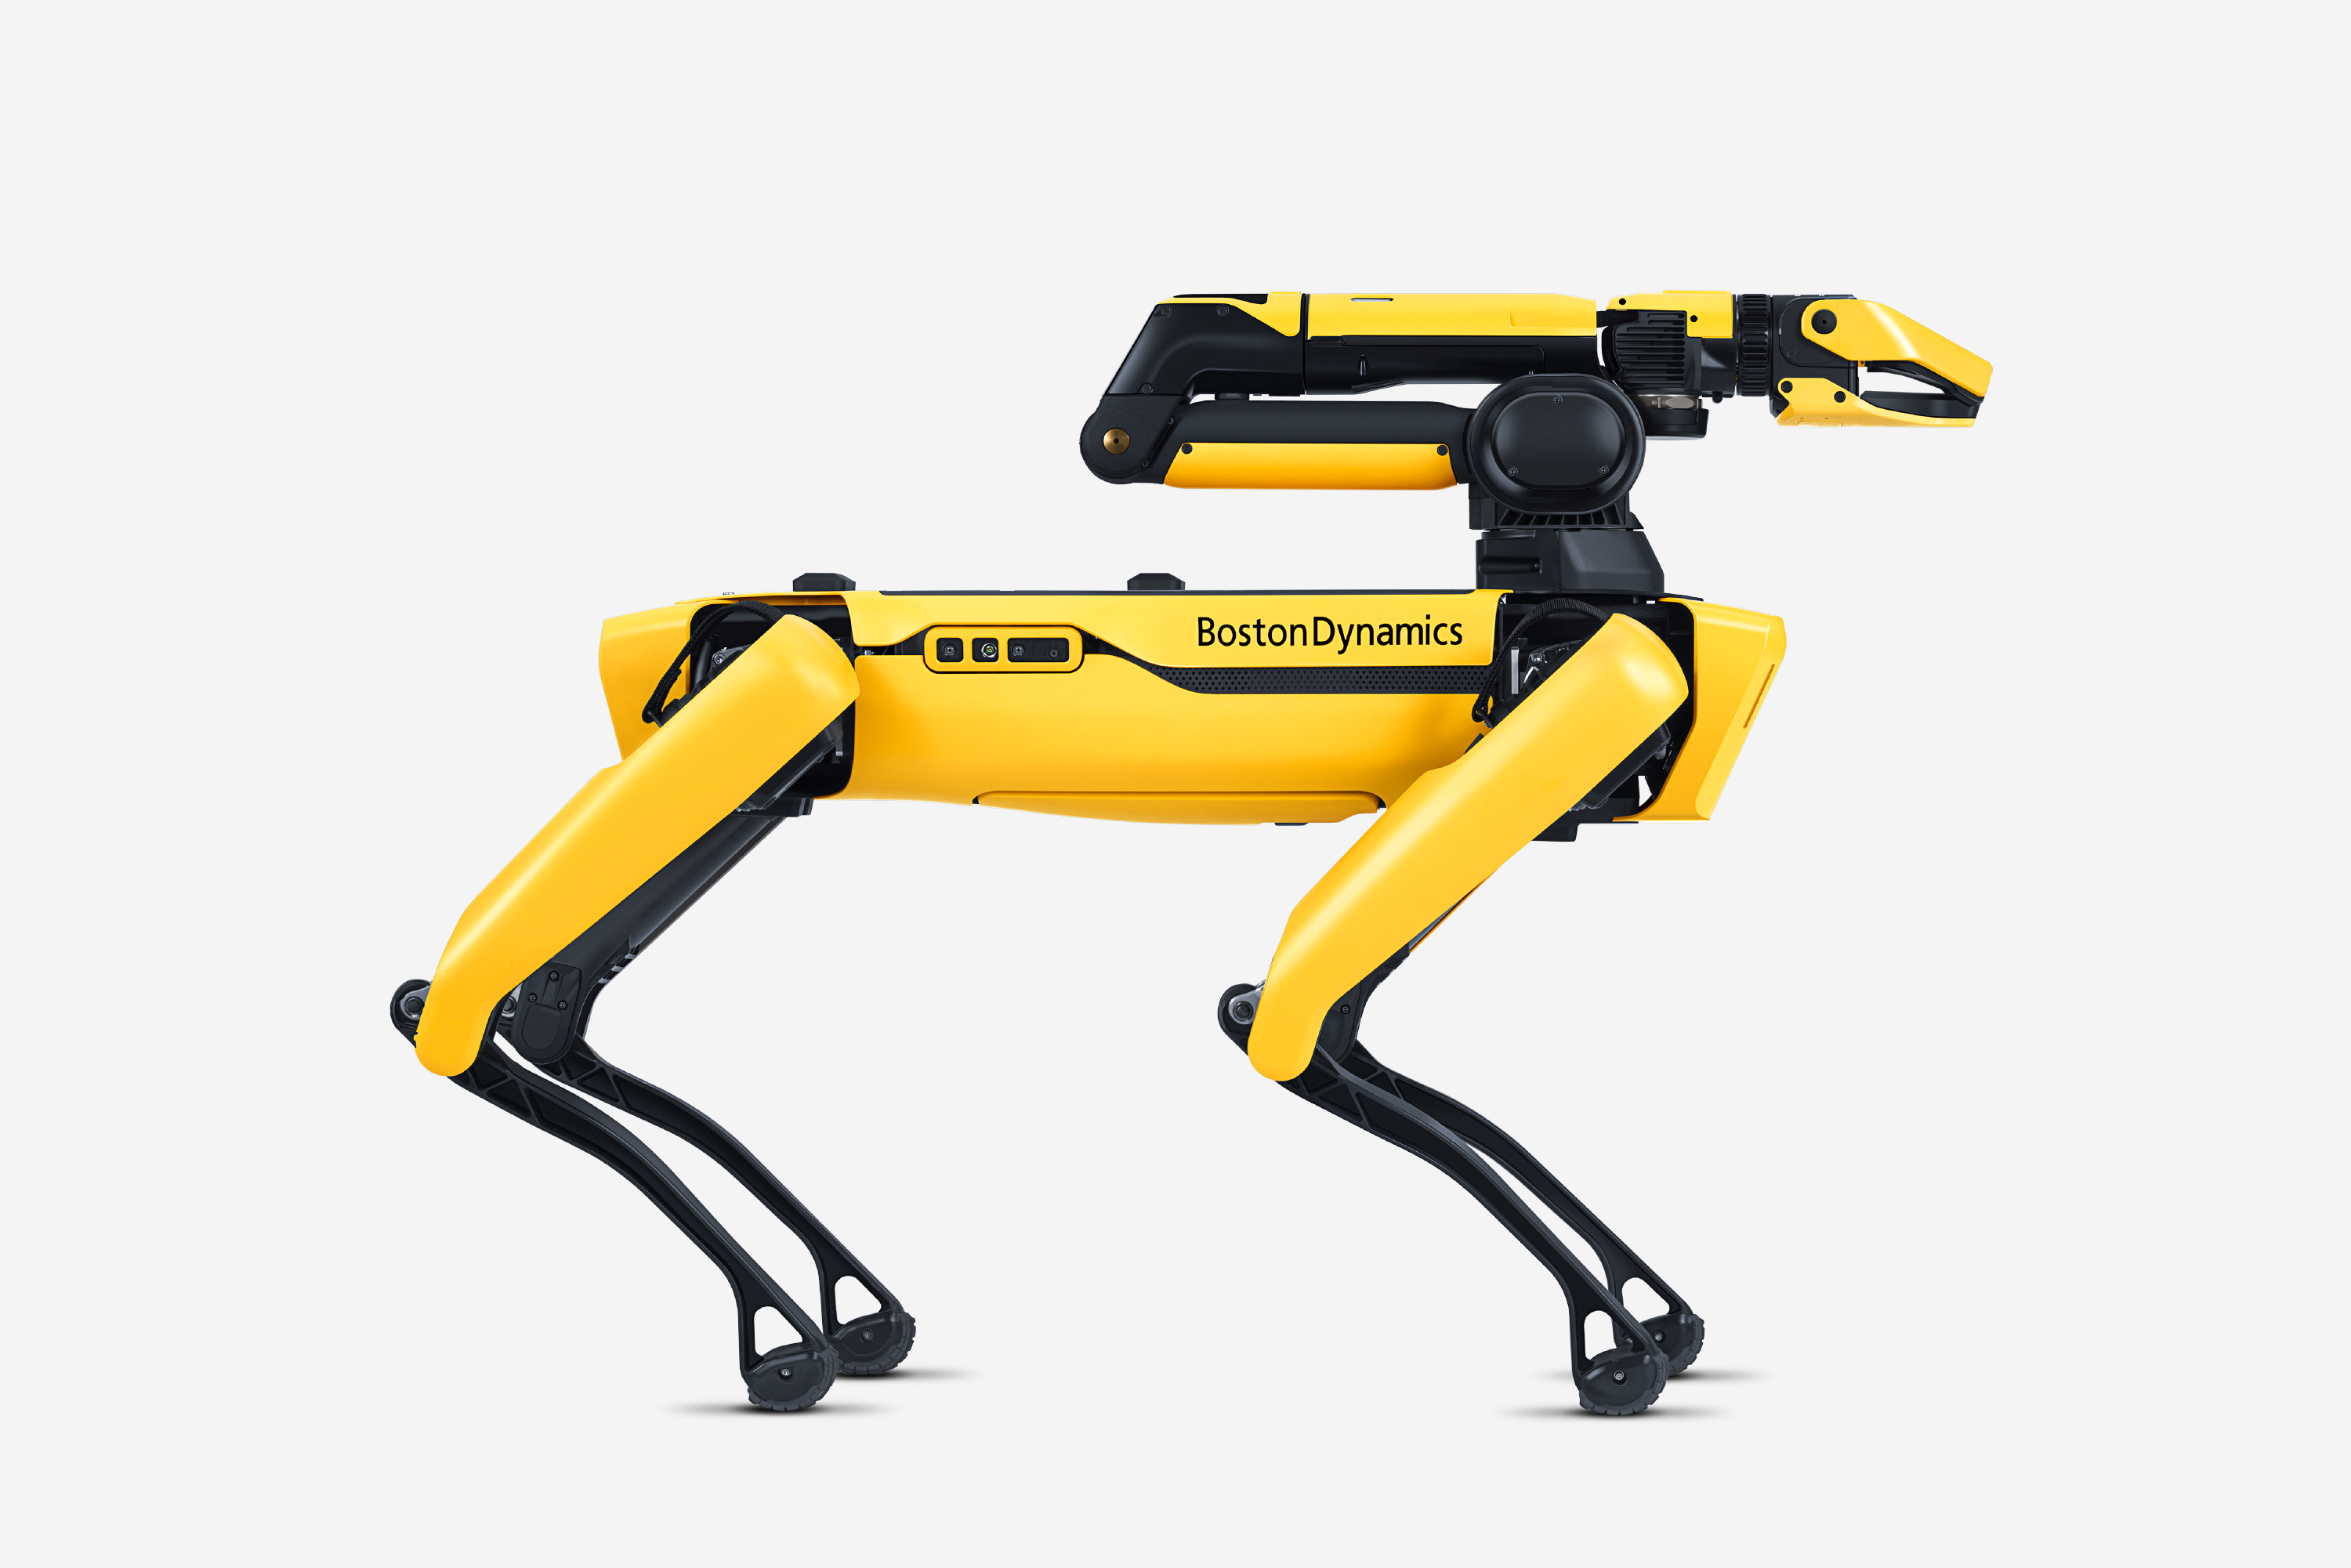
\includegraphics[scale=0.15]{figures/spot_arm.png}
  \caption{The Spot with Robot from Boston Dynamics []}
  \label{Fig:spot_arm}
\end{figure}

\\